\documentclass[tikz, margin=2mm, convert={density=300,size=1920x1080,outext=.png}]{standalone}

\usepackage[utf8]{inputenc}
\usetikzlibrary{shapes,arrows,calc}
\tikzstyle{box} = [rectangle, minimum width=2cm, text width=6em, text centered, rounded corners, minimum height=1cm, draw=black]
\tikzstyle{arrow} = [draw, -latex']
\begin{document}
    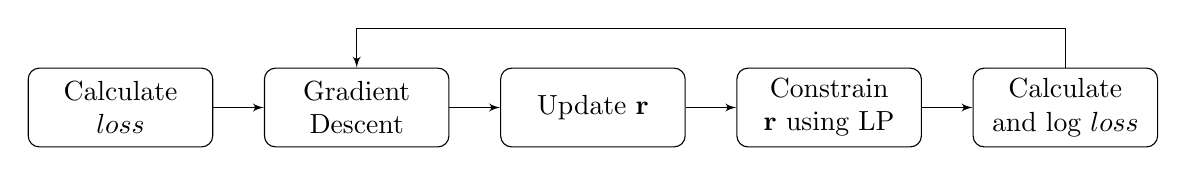
\begin{tikzpicture}[node distance=3cm, auto]
        \node (calcLoss) [box] {Calculate $loss$};
        \node (gd) [box, right of=calcLoss] {Gradient Descent};
        \node (update) [box, right of=gd] {Update $\mathbf{r}$};
        \node (constrain) [box, right of=update] {Constrain $\mathbf{r}$ using LP};
        \node (calcLossLog) [box, right of=constrain] {Calculate and log $loss$};
        
        \path [arrow] (calcLoss) -- (gd);
        \path [arrow] (gd) -- (update);
        \path [arrow] (update) -- (constrain);
        \path [arrow] (constrain) -- (calcLossLog);
        \path [arrow] (calcLossLog) |- ($(gd.north) + (0, 0.5)$) -- (gd);
    \end{tikzpicture}
\end{document}